\documentclass[aspectratio=169]{beamer}
\usetheme[theline=0.92]{CITIUS}

%% Imports
\usepackage[utf8]{inputenc}
\usepackage{lipsum}
\usepackage{multirow}
\usepackage[spanish,es-nodecimaldot]{babel}
\usepackage[backend=bibtex,style=numeric]{biblatex} % or style=authoryear, etc.
\addbibresource{references.bib}  % Make sure the file name matches your .bib file
\usepackage{subcaption}
%% Definitions
\title{Aplicación de curvas de llenado del espacio en nubes \\ de puntos 3D almacenadas en Octrees}
%\subtitle{A modern approach}
\author{Pablo Díaz, Miguel Yermo, José C. Cabaleiro, Francisco F. Rivera}
\date{Junio 2025}
\def\toctitle{Índice}


% COLORES OCTREES

% Define custom colors (RGB or HEX-like via HTML)
\definecolor{octUnencoded}{HTML}{E1A692}
\definecolor{octMort}{HTML}{DE6E56}
\definecolor{octHilb}{HTML}{C23728}
\definecolor{loctMort}{HTML}{63BFF0}
\definecolor{loctHilb}{HTML}{1984C5}
% Macros for colored bullets with spacing
\newcommand{\dotUnencoded}{\textcolor{octUnencoded}{\textbullet}~}
\newcommand{\dotOctMort}{\textcolor{octMort}{\textbullet}~}
\newcommand{\dotOctHilb}{\textcolor{octHilb}{\textbullet}~}
\newcommand{\dotLoctMort}{\textcolor{loctMort}{\textbullet}~}
\newcommand{\dotLoctHilb}{\textcolor{loctHilb}{\textbullet}~}

%% Uncomment for outline before each section
% \AtBeginSection[] {
%    \begin{frame}[plain]{\toctitle}
%        \tableofcontents[currentsection]
%    \end{frame}
% }

\begin{document}

%% Title page
\begin{frame}[plain]%
    \titlepage%
    
\end{frame}
  
%% Outline page
\begin{frame}[plain]{\toctitle}
    \tableofcontents
\end{frame}
\setcounter{framenumber}{0} %% To count only pages with content

\section{Búsquedas de vecinos}

\begin{frame}{Búsquedas de vecinos}

Dada una nube de puntos tridimensional $\mathcal{P}$, un centro $c$ y un radio $r$, buscamos encontrar todos los puntos $q \in \mathcal{P}$ con $\left\lVert q-c \right\rVert < r$.

Esta operación extrae la estructura local de la nube, y tiene innumerables usos en el procesado de nubes de puntos: clusterización, segmentación, extracción de propiedades, etc.
% METER DIAGRAMA BÚSQUEDA DE VECINOS / KERNEL
\vspace{2em}

\textbf{Problema:} extraer los vecinos de un gran número de puntos es costoso, y de hecho suele ser la parte más computacionalmente demandante del procesado de la nube.
\end{frame}

\begin{frame}{Nubes LiDAR}
    \begin{columns}
        \column{0.5\textwidth}
            \begin{itemize}
                \item Gran tamaño, altamente irregulares tanto en densidad como en geometría
                \item Varios tipos (sensor aéreo vs terrestre)
                \item Necesidad de algoritmos y estructuras de datos optimizados para el cálculo de vecinos
            \end{itemize}        
        \column{0.5\textwidth}
        \begin{figure}
            \centering
            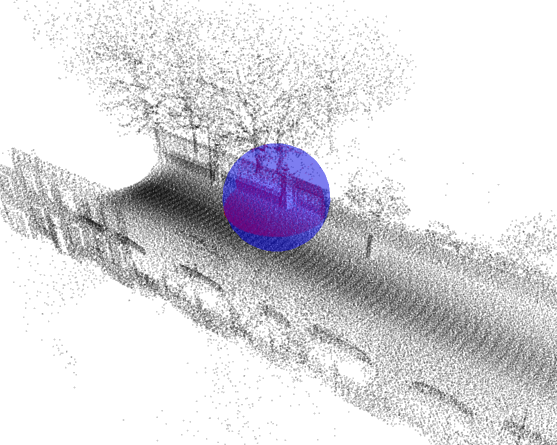
\includegraphics[scale=0.65]{img/vecindario_lille.png}
            \caption{Vecindario esférico en la nube \textit{Lille\_0}}
        \end{figure}
    \end{columns}
\end{frame}

\section{Curvas de llenado del espacio (SFCs)}
\begin{frame}{Curvas de llenado del espacio}
    \begin{itemize}
        \item Normalmente, los datos de las nubes se almacenan como un vector de puntos, en el mismo orden de escaneo del sensor LiDAR $\rightarrow$ \textbf{Mala localidad espacial} 
        \item Puntos muy cercanos en el espacio tridimensional pueden encontrarse muy alejados en memoria
        \item ¿Cómo mejorar la localidad? $\rightarrow$ Reordenando la nube mediante una curva de llenado del espacio \textit{(\textbf{S}pace \textbf{F}illing \textbf{C}urve)} \cite{asano1997space}
    \end{itemize}
% Poner figura con Nube sin reordenar -> curva -> nube reordenada (abajo del texto para variar)
\end{frame}

\begin{frame}{SFCs de Morton y Hilbert}
    \begin{columns}
        \column{0.5\textwidth}
            \textbf{SFC de Morton} \cite{morton1966computer}
            % IMAGEN CURVA      
            \begin{itemize}
                \item Presenta saltos, menor localidad
                \item Cálculo en unas pocas instrucciones (LUTs, vectorización)
            \end{itemize}
            \begin{figure}
                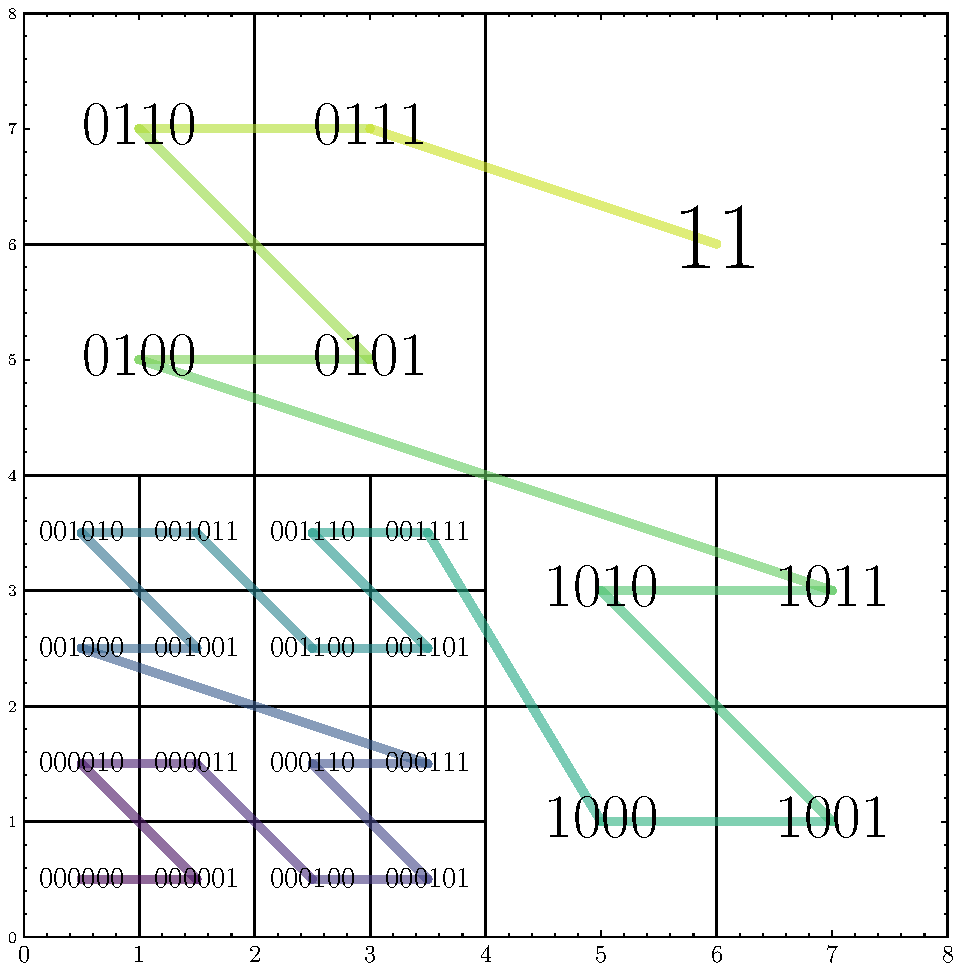
\includegraphics[scale=0.27]{img/morton_quadtree.pdf}
            \end{figure}
        \column{0.5\textwidth}
            \textbf{SFC de Hilbert} \cite{lam1994class,miki2017gothic}
            % IMAGEN CURVA   

            \begin{itemize}
                \item Continua, mejor localidad teórica (continuidad en ${\left\lVert \cdot \right\rVert}_\infty$)
                \item Cálculo iterativo más lento
            \end{itemize}            
            \begin{figure}
                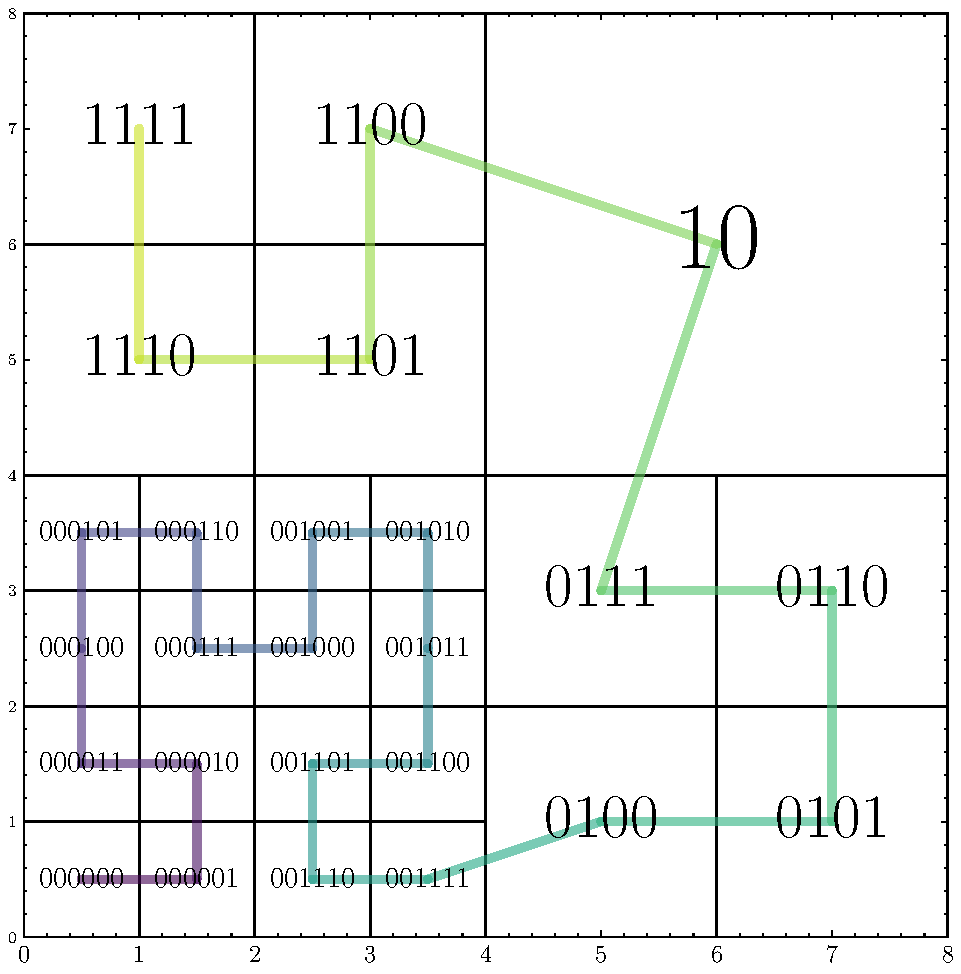
\includegraphics[scale=0.27]{img/hilbert_quadtree.pdf}
            \end{figure}
        \end{columns}
\end{frame}

\begin{frame}{Reordenando la nube}
    \begin{enumerate}
        \item Discretización: hallar la \textit{bounding box} y trasladar todos los puntos al espacio $S_L = [0,2^L) \times [0, 2^L) \times [0, 2^L) \subset \mathbb{Z}^3$.
        \item Para cada punto $p =(x,y,z) \in S_L$, hallar su código $c$ de Morton o de Hilbert de $3L$ bits, marcando su orden en la curva de profundidad $L$.
        \item Una vez se han hallado todos los códigos, utilizarlos como índice para reordenar la nube.
    \end{enumerate}

\end{frame}

\begin{frame}{Reordenando la nube}
    \begin{figure}
        \centering
        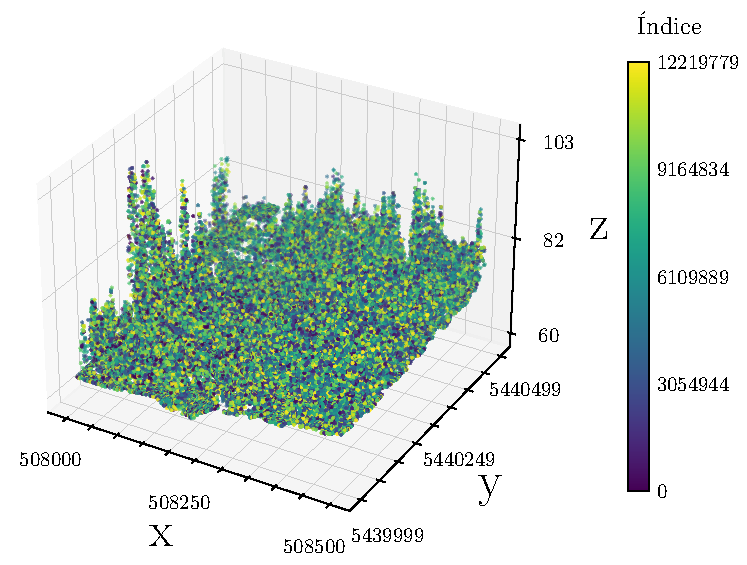
\includegraphics[width=0.55\textwidth]{img/plot_5080-54400_unencoded.pdf}
        \caption{Nube original del dataset \textit{DALES}, con color según orden de índices.}
    \end{figure}
\end{frame}

\begin{frame}{Reordenando la nube}
    \begin{figure}
        \centering
        \begin{subfigure}{0.45\textwidth}
            \centering
            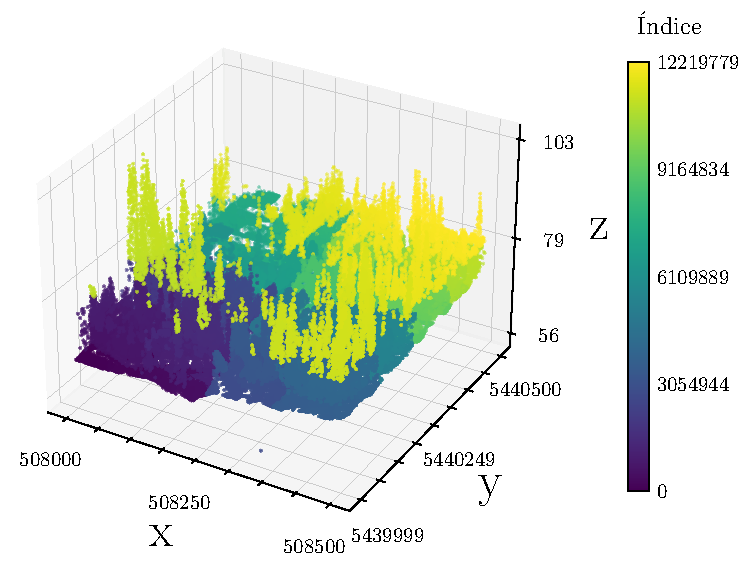
\includegraphics[width=\linewidth]{img/plot_5080-54400_morton.pdf}
            \caption{Reordenada (Morton)}
        \end{subfigure}
        \hfill
        \begin{subfigure}{0.45\textwidth}
            \centering
            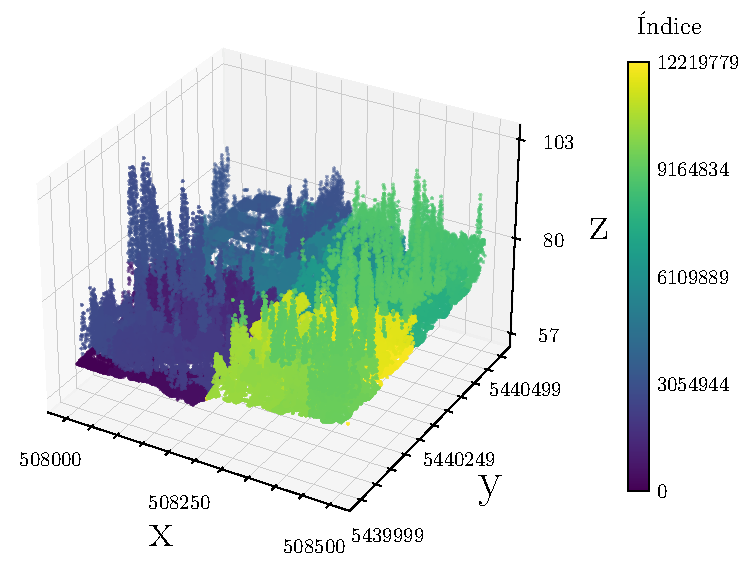
\includegraphics[width=\linewidth]{img/plot_5080-54400_hilbert.pdf}
            \caption{Reordenada (Hilbert)}
        \end{subfigure}
        \caption{Nube reordenada con dos técnicas distintas.}
    \end{figure}
\end{frame}


\section{Octrees}
\begin{frame}{Octrees}
    \begin{columns}
        \column{0.5\textwidth}    
        \begin{enumerate}
            \item Estructura jerárquica de volúmenes (\textit{BVH}) donde el espacio se subdivide recursivamente en $8$ octantes.
            \item Los nodos internos tienen 8 suboctantes, las hojas tienen puntos de la nube. 
            \item Se subdivide hasta que las hojas no tienen más de $N_{max}$ puntos.
        \end{enumerate}
        \vspace{0.8em}

        \begin{block}{\textbf{¿Cómo almacenar los nodos?}}
            \textrightarrow \: Octrees basados en punteros \\
            \textrightarrow \: Octrees lineales
        \end{block}
        \column{0.5\textwidth}
        \begin{figure}[t]
            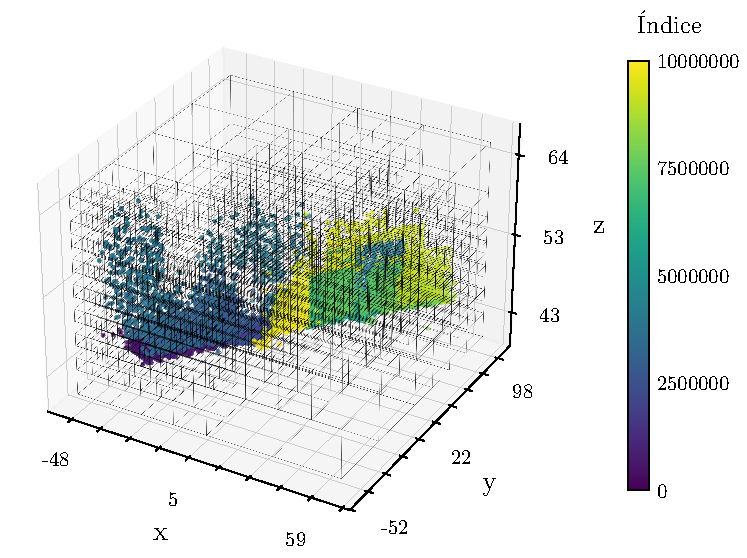
\includegraphics[scale=0.55]{img/plot_Lille_0_hilbert_oct.pdf}
            \caption{Construcción de un Octree sobre la nube Lille\_0, reordenada mediante la curva de Hilbert}
        \end{figure}
        % PONER IMAGEN OCTREE Y OCTREE BASADO EN PUNTEROS?
    \end{columns}
    
\end{frame}

\begin{frame}{Búsqueda de vecinos en Octrees}
    \begin{columns}
    \column{0.5\textwidth}
    % TODO meter algo
    \textit{Algoritmo de búsqueda en profundidad}
    \vspace{1em}
        \begin{enumerate}
            \item Si el nodo es una rama, calculamos su posición relativa respecto al \textit{kernel}:
            \begin{enumerate}
                \item[1a.] Octante interseca al \textit{kernel} \textrightarrow\: Seguir descendiendo.
                \item[1b.] Octante fuera del \textit{kernel} \textrightarrow\:  Parar.
            \end{enumerate}
            \item Si llegamos a una hoja, comprobamos punto a punto si pertenecen o no al \textit{kernel} propuesto. 
            \item Finalmente, devolvemos todos los puntos en el interior del \textit{kernel}.
        \end{enumerate}
        \column{0.5\textwidth}
        \begin{exampleblock}{Ventajas}
            % No creo que haga mucha falta apuntar que es log N
            \textrightarrow \: Mucho mejor que fuerza bruta: $\mathcal{O}(\log{N})$ en vez de $\mathcal{O}(N)$. \\
            \textrightarrow \: Los puntos de las hojas están próximos en memoria gracias a las SFCs. \\
        \end{exampleblock}
        \begin{alertblock}{Desventajas}
            \textrightarrow \: Se debe recorrer el árbol hasta las hojas \\
            \textrightarrow \: Muchas redirecciones de punteros, peor localidad del árbol \\
        \end{alertblock}
    \end{columns}
\end{frame}

\begin{frame}{Optimización con Octrees lineales}
        El Octree lineal propuesto es una variante de la estructura \textit{cornerstone-octree} dada por Keller et al. \cite{Keller2023}, originalmente usada en simulaciones de partículas.
        \vspace{1em}
        \begin{block}{Ideas principales}
            \textrightarrow \: Cada hoja o nodo interno se puede representar mediante el \textbf{rango de índices} de la nube reordenada, gracias al reordenamiento por SFCs. \\
            \textrightarrow \: La información para enlazar el árbol y realizar las búsquedas también se puede comprimir en un array indicando el primer hijo de cada octante.
        \end{block} 

        \textbullet\: Por ejemplo, bajo el $i$-ésimo hijo del nodo raíz ($0 \leq i \leq 7$) tenemos los puntos con SFC en $[i\cdot 8^{3L-1}, (i+1) \cdot 8^{3L-1})$, con índices en el rango $[a_i, a_{i+1})$, siendo $a_0 = 0$ y $a_8 = N$.
\end{frame}

\begin{frame}
    \begin{columns}
        \column{0.5\textwidth}    
        El Octree lineal cuenta con las siguientes características:
        \begin{enumerate}
            \item Construcción rápida y altamente paralelizable.
            \item \textbf{Rangos de índices en la rama disponible en todos los nodos, y consecutivos gracias a las SFCs.}
            \item Estructura compacta y contenida en unos pocos arrays: muy buena localidad y poco overhead en memoria.
        \end{enumerate}
        \column{0.5\textwidth}
        \textit{Algoritmo optimizado de búsquedas}
        \vspace{1em}
        \begin{enumerate}
            \item Si el nodo es una rama, calculamos su posición relativa respecto al \textit{kernel}:
              \begin{enumerate}
                    \item[1a.] \textbf{Octante contenido en \textit{kernel} \textrightarrow\: Insertar puntos secuencialmente, usando la estructura lineal con acceso directo a los puntos.}
                   \item[1b.] Octante interseca al \textit{kernel} \textrightarrow\: Seguir descendiendo.
                   \item[1c.] Octante fuera del \textit{kernel} \textrightarrow\:  Parar.
              \end{enumerate}
            \item Si llegamos a una hoja, comprobamos punto a punto si pertenecen o no al \textit{kernel} propuesto. 
            \item Finalmente, devolvemos todos los puntos en el interior del \textit{kernel}.
        \end{enumerate}
    \end{columns}

\end{frame}
\section{Resultados}
\begin{frame}{Configuración experimental}
    Conjunto de nubes variado: \textit{Paris-Lille}, \textit{DALES}, \textit{Semantic3D} y \textit{Speulderbos}. % TODO meter características más básicas nubes (tamaño y terrestre vs aérea)

    \textrightarrow \: 2 experimentos principales:
    \begin{enumerate}
        \item \textbf{Búsquedas aleatorias:} $5000$ búsquedas en un subconjunto de centros aleatorio $v_c \subset P$, con varios radios, \textit{kernels} (esfera, círculo, cubo, cuadrado) y combinaciones SFC+Octree. 
        \item \textbf{Búsquedas completas:} lo mismo pero con $v_c = P$, y realizando las búsquedas con el orden de la nube tras el reordenamiento, para más localidad.
    \end{enumerate}
    \textrightarrow \: Paralelización a nivel de bucle con OpenMP, 40 hilos sobre arquitectura NUMA.

    \begin{table}
    
        \begin{tabular}{@{}lll@{}}
            \textbf{Octree} & \textbf{Reordenamiento} & \textbf{Nombre} \\
            \hline
            Punteros        & Ninguno       & \dotUnencoded \texttt{poct\_unsorted} \\
                            & Morton        & \dotOctMort \texttt{poct\_mort} \\
                            & Hilbert       & \dotOctHilb \texttt{poct\_hilb} \\
            \hline
            Lineal          & Morton        & \dotLoctMort \texttt{loct\_mort} \\
                            & Hilbert       & \dotLoctHilb \texttt{loct\_hilb} \\
        \end{tabular}
    \end{table}
\end{frame}

\begin{frame}{Resultados}
    \vspace{-1em} % Optional: Pull up if needed
    \begin{columns}[t] % Align top for better fitting
        \column{0.5\textwidth}
        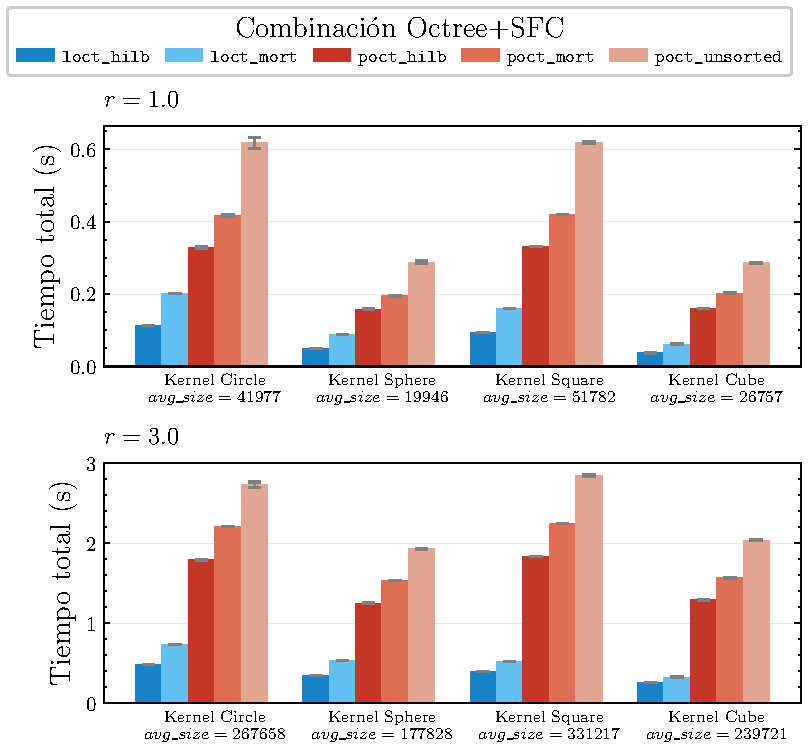
\includegraphics[width=0.8\linewidth]{img/paris_luxembourg_6_subsets_reduced.pdf}
        {\scriptsize \centering Búsquedas aleatorias - Tiempos en \textit{Paris\_Luxembourg\_6}, para $r=1.0m$ y $r=3.0m$ y varios kernels \par}

        \column{0.5\textwidth}
            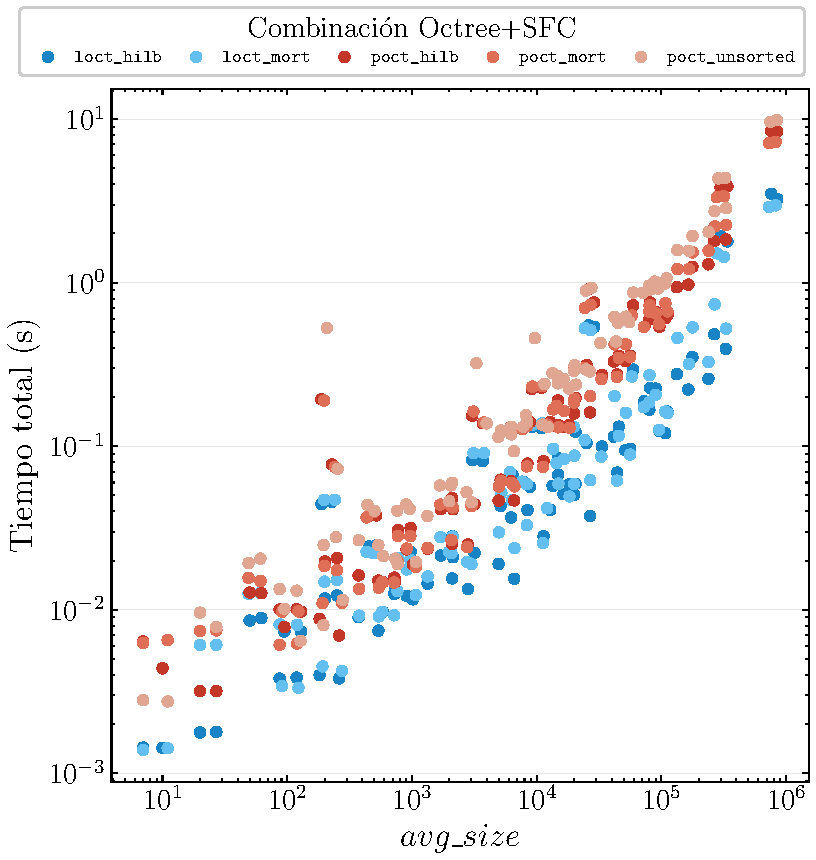
\includegraphics[width=0.8\linewidth]{img/loglog_subsets.pdf}
            {\scriptsize \centering Búsquedas aleatorias - Tiempo vs tamaño promedio de los vecindarios en varias nubes (log-log) \par}    \end{columns}
\end{frame}

\begin{frame}{Resultados}
    \begin{columns}
    \column{0.2\textwidth}
    \textit{Búsquedas completas - Varias nubes, kernel esférico}
    \column{0.8\textwidth}
    \vspace{-0.5em} 
        \begin{table}
            \scriptsize
            \begin{tabular}{|c|c|c|ccc|}
            \hline
            Nube                      & $n$                    & $r$ (m)                  & Octree                    & SFC     & Tiempo (s)\\ \hline
            \multirow{5}{*}{\textit{Lille\_0}} & \multirow{5}{*}{10.00M} & \multirow{5}{*}{3.0} & \multirow{3}{*}{Punteros} & - & 445.24 \\
            &  &  &  & Morton & 332.11 \\
            &  &  &  & Hilbert & 324.87 \\ \cline{4-6}
            &  &  & \multirow{2}{*}{Lineal} & Morton & 130.96 \\
            &  &  &  & Hilbert & \textbf{130.20} \\
            \hline
            \multirow{5}{*}{\textit{5080\_54400}} & \multirow{5}{*}{12.22M} & \multirow{5}{*}{10.0} & \multirow{3}{*}{Punteros} & - & 98.04 \\
            &  &  &  & Morton & 64.99 \\
            &  &  &  & Hilbert & 62.80 \\ \cline{4-6}
            &  &  & \multirow{2}{*}{Lineal} & Morton & \textbf{42.66} \\
            &  &  &  & Hilbert & 46.31 \\
            \hline
            \multirow{5}{*}{\textit{bildstein\_station1}} & \multirow{5}{*}{29.70M} & \multirow{5}{*}{0.1} & \multirow{3}{*}{Punteros} & - & 118.44 \\
            &  &  &  & Morton & 106.35 \\
            &  &  &  & Hilbert & 103.08 \\ \cline{4-6}
            &  &  & \multirow{2}{*}{Lineal} & Morton & \textbf{60.66} \\
            &  &  &  & Hilbert & 65.11 \\
            \hline
            \multirow{5}{*}{\textit{sg27\_station8}} & \multirow{5}{*}{429.62M} & \multirow{5}{*}{0.05} & \multirow{3}{*}{Punteros} & - & 2549.36 \\
            &  &  &  & Morton & 2243.24 \\
            &  &  &  & Hilbert & 2208.13 \\ \cline{4-6}
            &  &  & \multirow{2}{*}{Lineal} & Morton & \textbf{1273.68} \\
            &  &  &  & Hilbert & 1427.66 \\
            \hline
            \end{tabular}
        \end{table}
    \end{columns}
\end{frame}

\begin{frame}{Conclusiones}
    \begin{itemize}
        \item El reordenamiento por curvas de Morton y Hilbert mejora la localidad de la nube, lo cuál reduce el tiempo de las búsquedas.
        \item La implementación empleada para el Octree lineal aporta una mejora muy considerable frene a la estructurada basada en punteros.
        \item La reordenación mediante SFCs y el Octree lineal tienden a mejorar el coeficiente de paralelización de las búsquedas.
    \end{itemize}
\end{frame}

\begin{frame}{Últimos avances y trabajo futuro}
    \textrightarrow~Últimos avances:
    \begin{itemize}
        \item Método de búsqueda en Octree lineal devolviendo rangos de índices en vez de lista de punteros / índices \textrightarrow \: Gran mejora para $r$ grande.
        \item Mejorada la comprobación geométrica para kernels esféricos, a partir del trabajo de Behley et al. \cite{behley2015efficient}
        \item Con todo esto, búsquedas mucho más rápidas ($\approx 10x$) que los Octrees y KD-Trees de PCL y $2-3x$ veces más rápidas que el Octree desarrollado por Behley et al. \cite{behley2015efficient}
    \end{itemize}

    \textrightarrow~Trabajo futuro:

    \begin{itemize}
        \item Probar búsquedas $k$-NN.
        \item Comparar con más librerías.
        \item Profiling de memoria.
        \item \dots
    \end{itemize}
\end{frame}



% \begin{frame}
% \frametitle{Pictures}
% \begin{figure}
% \includegraphics[scale=0.5]{img/logo_CiTIUS}
% \caption{CITIUS Logo}
% \end{figure}
% \end{frame}

% \begin{frame}{Hyperlinks and Buttons}
% \hyperlink{contents}{contents page}
% Here are some other button commands we can use.

% \hyperlink{columns}{\beamergotobutton{columns page}}

% \hyperlink{pictures}{\beamerskipbutton{pictures page}}

% \hyperlink{pictures}{\beamerreturnbutton{pictures page}}
% \end{frame}
\setbeamertemplate{background}{
    \begin{tikzpicture}
        \node[opacity=.8,inner sep=0pt]{
            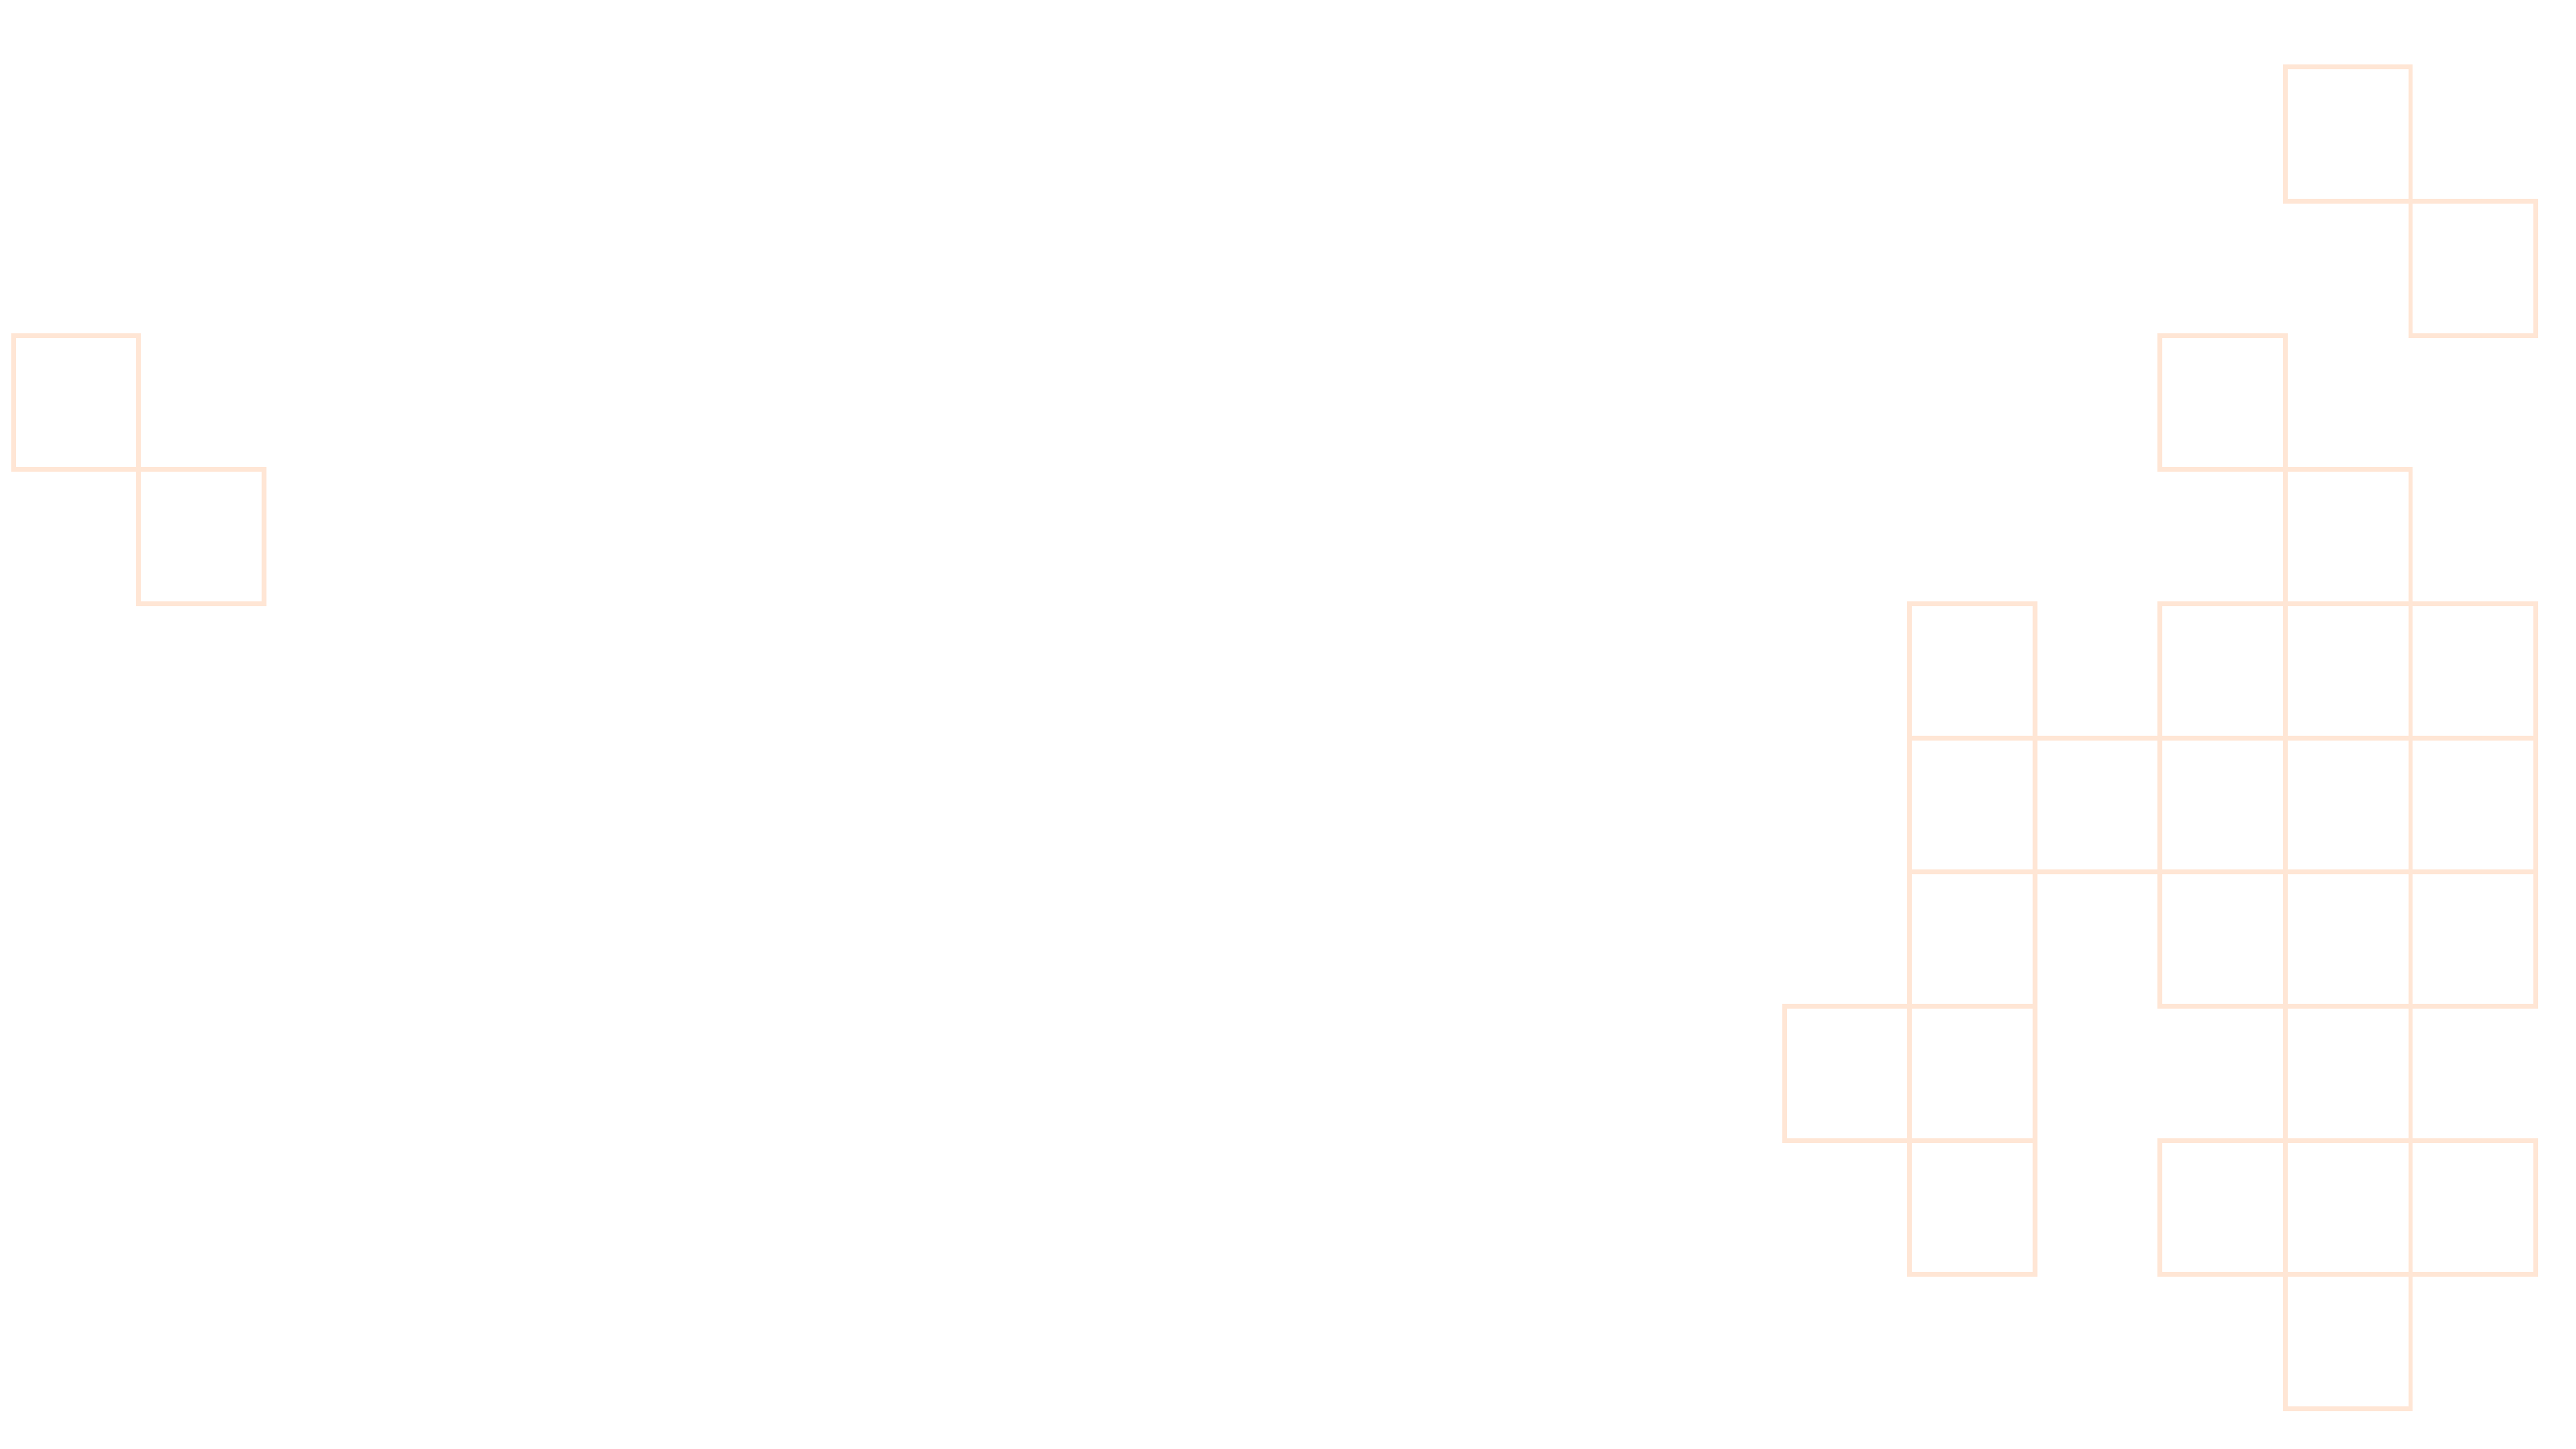
\includegraphics[height=\paperheight,width=\paperwidth]{img/background.pdf}};
    \end{tikzpicture}
}
\begin{frame}[plain,noframenumbering]
    \begin{center}
    \begin{minipage}{.75\textwidth}%
        \begin{beamercolorbox}[sep=1em, rounded=false, center]{header citius}%
            \Huge Preguntas?\vspace*{-1ex}%
        \end{beamercolorbox}%
    \end{minipage}
    \\[5pt]
    % \hyperlink{mailto:pablo.diaz.vinambres@rai.usc.es}{pablo.diaz.vinambres@rai.usc.es}

    % \bigskip

    % \begin{tikzpicture}
    %     \node[inner sep=10pt]{
    %         
\includegraphics[height=0.15\paperheight]{img/logos_FEDER_2014-2020.pdf}};
    % \end{tikzpicture}\\
    % Fondo Europeo de Desenvolvemento Rexional\\*
    % ``Unha maneira de facer Europa``
  \end{center}

\end{frame}

\begin{frame}[allowframebreaks]{Referencias}
    \printbibliography
\end{frame}

\end{document}
